% !TEX root =  thesis.tex
%-------------------------------Kopf----------------------------------
\ \\[-1cm]
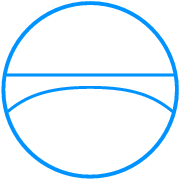
\includegraphics[height=1.5cm]{../pictures/Logos/bauiverm_blau_cut}
\rule{5mm}{0pt}
%
\includegraphics[height=1.5cm]{../pictures/Logos/CiE-Logo}
% TODO: CMS logo
\hfill

\includegraphics[height=1.5cm]{../pictures/Logos/TUMLogo_oZ_Vollfl_blau_RGB}
%
\includegraphics{../pictures/Logos/TUMLogo_oZ_Outline_blau_RGB}
\\[0.75cm]
{\large Department of Civil, Geo and Environmental Engineering\\[0.5ex]
Chair for Computation in Engineering\\
Prof. Dr.-Ing. André Borrmann}
\ \\[13ex]
%---------------------------------Thema und Autor--------------------------------
%%%%%%%%%%%%%%
\begin{center}
\begin{spacing}{2.0}
	{\color{tumblue}{\huge{\bf{\DAthema}}}} \ \\[7ex]
\end{spacing}
{\Large{\bf{\DAautor}}}\\[5ex]
\vfill
{\Large{{\DAtype}}}\\[6ex]
%-----------------------------weitere Angaben -----------------------------------
\newcolumntype{L}[1]{>{\raggedright\let\newline\\\arraybackslash\hspace{0pt}}m{#1}}
\newcolumntype{C}[1]{>{\centering\let\newline\\\arraybackslash\hspace{0pt}}m{#1}}
\newcolumntype{R}[1]{>{\raggedleft\let\newline\\\arraybackslash\hspace{0pt}}m{#1}}
\renewcommand{\arraystretch}{1.2}
\begin{tabular}{R{0.47\textwidth} L{0.50\textwidth}}
Author:               & \DAautor     \\
Matriculation number: & \Matrikel    \\
Supervisor:           & \DAprofessor \\
Advisor:              & \DAbetreuer  \\
Date of issue:        & \DAausgabe   \\
Date of submission:   & \DAabgabe    \\
\end{tabular}
\end{center}
%-----------------------
\cleardoublepage
